
\documentclass[border=10pt]{standalone}

\usepackage{tikz}
\usetikzlibrary{fit,positioning,calc}


%default strings

\begin{document}
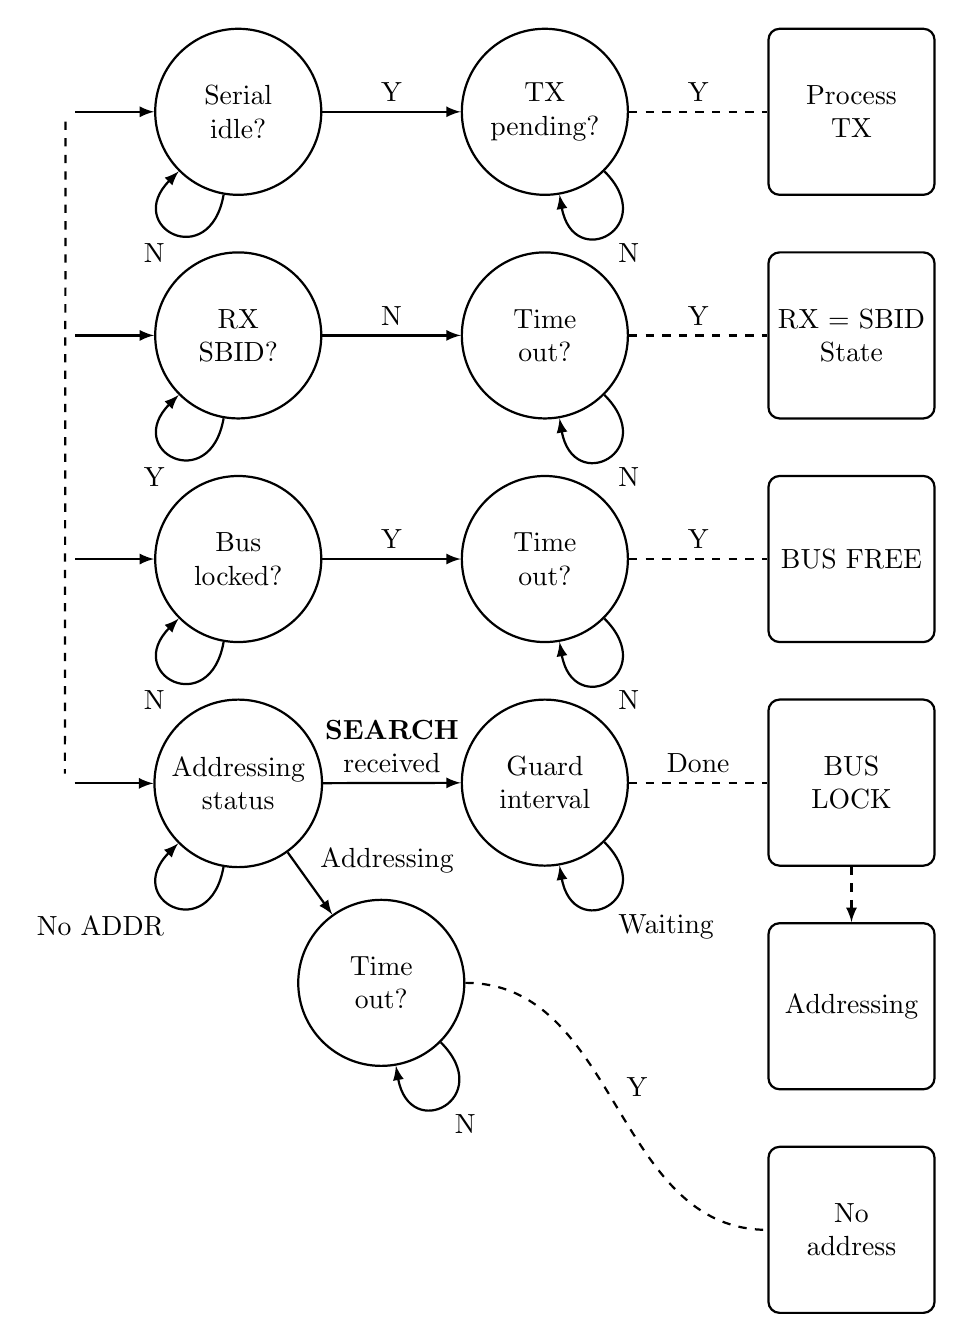
\begin{tikzpicture}[auto]

\tikzstyle{stackitem}=[rounded corners,align=center,thick,circle,minimum size=60pt,draw=black, node distance=20pt]
\tikzstyle{process}=[rounded corners,align=center,thick,rectangle,minimum size=60pt,draw=black, node distance=20pt]


\node [stackitem] (sidle) {Serial \\ idle?};
\node [stackitem, right= of sidle,xshift=30pt] (txpend) {TX \\ pending?};

\node[stackitem,below= of sidle] (rxsbid) {RX \\ SBID?};
\node[stackitem,below= of txpend] (timeout) {Time \\ out?};

\node[stackitem,below= of rxsbid] (buslock) {Bus \\ locked?};
\node[stackitem,below= of timeout] (timeout2) {Time\\ out?}; 

\node[stackitem,below= of buslock] (addrstat) {Addressing \\ status};
\node[stackitem,below= of timeout2] (guard) {Guard\\ interval};

\path [-latex,thick] (sidle) edge node {Y} (txpend)
      [-latex,thick] (rxsbid) edge node {N} (timeout) 
      [-latex,thick] (buslock) edge node {Y} (timeout2) 
      [-latex,thick] (addrstat) edge node [align=center] {\textbf{SEARCH} \\ received} (guard);

\path [-latex,thick] (sidle) edge [out=260, in=225,looseness=4] node {N} (sidle)
 [-latex,thick] (rxsbid) edge [out=260, in=225,looseness=4] node {Y} (rxsbid)
 [-latex,thick] (buslock) edge [out=260, in=225,looseness=4] node {N} (buslock)
 [-latex,thick] (addrstat) edge [out=260, in=225,looseness=4] node {No ADDR} (addrstat);

\path [-latex,thick] (txpend) edge [out=315, in=280,looseness=4] node {N} (txpend)
 [-latex,thick] (timeout) edge [out=315, in=280,looseness=4] node {N} (timeout)
 [-latex,thick] (timeout2) edge [out=315, in=280,looseness=4] node {N} (timeout2)
 [-latex,thick] (guard) edge [out=315, in=280,looseness=4] node {Waiting} (guard);

\node[process,right= of txpend,xshift=30pt] (proctx) {Process\\ TX};
\node[process,below= of proctx] (proc2) {RX = SBID \\ State};
\node[process,below= of proc2] (proc3) {BUS FREE};
\node[process,below= of proc3] (proc4) {BUS \\ LOCK};
\node[process,below= of proc4] (proc5) {Addressing};
\node[process,below= of proc5] (proc6) {No \\ address};

\path [dashed,thick] (txpend) edge node {Y} (proctx)
[dashed,thick] (timeout) edge node {Y} (proc2)
[dashed,thick] (timeout2) edge node {Y} (proc3)
[dashed,thick] (guard) edge node {Done} (proc4)
[-latex,dashed,thick] (proc4) edge (proc5);

\node[stackitem,below= of addrstat.south east,xshift=30pt] (timeout3) {Time \\ out?};

\path [-latex,thick] (addrstat) edge node {Addressing} (timeout3)
      [-latex,thick] (timeout3) edge [out=315,in=280,looseness=4] node {N} (timeout3);
\path [dashed,thick] (timeout3) edge [out=0,in=180] node {Y} (proc6);

\node [draw=none,left= of sidle] (invis1) {};
\node [draw=none,left= of rxsbid] (invis2) {};
\node [draw=none,left= of buslock] (invis3) {};
\node [draw=none,left= of addrstat] (invis4) {};
\path [-latex,thick] (invis1) edge (sidle)
      (invis2) edge (rxsbid)
      (invis3) edge (buslock)
      (invis4) edge (addrstat);

\path [dashed,thick] (invis1) edge (invis4);



\end{tikzpicture}
\end{document}